\chapter{Wybrane mechanizmy w języku Rust}
Niniejszy rozdział koncentruje się na analizie wybranych mechanizmów oferowanych przez język programowania Rust w kontekście współbieżności i równoległości. Omówione zostaną fundamentalne koncepcje, które stanowią o unikalności tego języka. Rozdział zawiera również analizę mechanizmów synchronizacyjnych oraz komunikacji międzywątkowej. Zawarte przykłady kodu ilustrują praktyczne zastosowania omawianych koncepcji i stanowią punkt odniesienia dla dalszych rozważań porównawczych.
\section{Podejście do współbieżności i równoległości}

Rozwój języka Rust oferuje szereg funkcji, które czynią go dobrym wyborem do programowania współbieżnego oraz równoległego. Kluczowymi elementami, które wyróżniają go na tle innych języków programowania są \cite{rustPolishNames}:
\begin{enumerate}
    \item Własność \eng {ownership} i pożyczanie \eng {borrow}: Model własności języka Rust zapewnia, że dane są bezpiecznie współdzielone między wątkami bez ryzyka wyścigów danych \eng{races}.
    \item Nieustraszona współbieżność \eng{fearless concurrency}: System typów Rusta wymusza reguły w czasie kompilacji, pozwalając programistom na pisanie współbieżnego kodu bez obawy o typowe pułapki.
    \item Inteligentne wskaźniki \eng{smart pointers}: Abstrakcje wspierające korzystanie oraz przesyłanie danych w programowaniu współbieżnym oraz równoległym.
\end{enumerate}

\subsection{Ownership oraz borrow}
\label{ownership_borrow}
Własność \eng {ownership} jest fundamentalnym konceptem w języku Rust, który zapewnia bezpieczeństwo pamięci bez konieczności stosowania mechanizmu odśmiecania \eng{garbage collection}. Każda wartość posiada jednego właściciela, który jest odpowiedzialny za zwolnienie pamięci zajmowanej przez tę wartość, gdy wychodzi ona z zakresu \eng{scope}. Model własności zapobiega wyścigom danych i zapewnia efektywne zarządzanie pamięcią.\\
Kluczowe zasady własności:
\begin{itemize}
    \item Każda wartość ma jednego właściciela.
    \item Gdy właściciel wychodzi z zakresu, wartość zostaje usunięta \eng{ropped}.
    \item Własność może zostać przeniesiona \eng{moved} na inną zmienną.
\end{itemize}

Pożyczanie \eng{borrowing} umożliwia tworzenie referencji do wartości bez przejmowania jej własności. Jest to kluczowe dla umożliwienia różnym częściom programu dostępu do danych bez ich duplikowania. Rust pozwala na pożyczanie wartości według dwóch zasad:
\begin{itemize}
    \item Pożyczanie niemutowalne (domyślne) \eng{immutable}: Można utworzyć wiele referencji, ale żadna z nich nie może modyfikować wartości.
    \item Pożyczanie mutowalne \eng{mutable}: W danym momencie może istnieć tylko jedna mutowalna referencja, co zapobiega wyścigom danych.
\end{itemize}
\begin{lstlisting}[language=Rust,caption=Przykład mechanizmu borrow, label=borrow_example]
fn main() {
    let s1 = String::from("Hello World");
    let s2 = &s1; // Immutable borrow - pożyczka niemutowalna
    println!("{}", s2); // Ok
    // let s3 = &mut s1; // Error
}
\end{lstlisting}
W powyższym listingu \ref{borrow_example} zaprezentowano element dotyczący użycia pożyczki w języku Rust. Błąd, oznaczony jako \texttt{Error} wynika z faktu, iż nie jest możliwe pożyczenie obiektu \texttt{s1} jako mutowalnego, ponieważ jest on jednocześnie pożyczany jako niemutowalny do obiektu \texttt{s2} (domyślnie).


\subsection{Nieustraszona współbieżność}
Mechanizm ten wynika bezpośrednio z rygorystycznych reguł systemu typów i modelu własności, które są integralną częścią tego języka. Dzięki temu Rust pozwala na tworzenie kodu współbieżnego, minimalizując ryzyko wystąpienia typowych błędów, takich jak wyścigi danych czy nieokreślone zachowanie wynikające z użycia wskaźników do już zwolnionej pamięci \eng{dangling pointers}.

Rust wymusza bezpieczeństwo współbieżności w czasie kompilacji poprzez analizę własności i okresu życia danych \eng{lifetimes}. Mechanizm ten zapobiega jednoczesnemu mutowalnemu dostępowi do tych samych danych w różnych wątkach (opisane w punkcie \ref{ownership_borrow}), co eliminuje potrzebę ręcznego zarządzania pamięcią czy synchronizacji przez programistę. Takie podejście czyni współbieżność w Rust nie tylko bezpieczną, ale również przewidywalną, co znacząco ułatwia jej implementację \cite{RustFC}.

\begin{figure}[H]
    \centering
    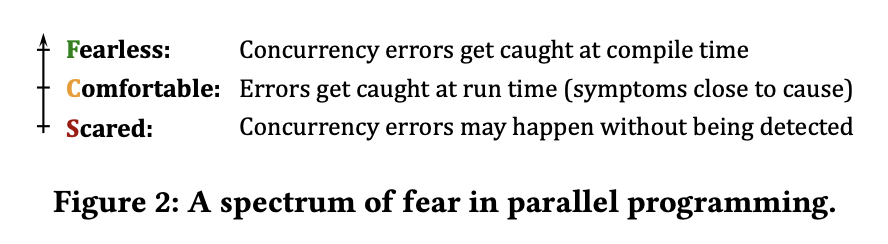
\includegraphics[width=0.6\linewidth]{images/FearlesRustExplain.png}
    \caption{Spektrum nieustraszonej współbieżności \cite{WhenIsParallelismFearlessandZeroCostwithRust?}}
    \label{fig:FearlessSpectrum}
\end{figure}
Autorzy \cite{WhenIsParallelismFearlessandZeroCostwithRust?}
uważają, że nieustraszona współbieżność jest lepiej interpretowana jako spektrum, zilustrowane na \ref{fig:FearlessSpectrum} idealnie eliminując wszelkie obawy przed błędami współbieżności w~czasie kompilacji (\texttt{Fearless}), ale jeśli nie jest to możliwe, utrzymując objawy błędów w~czasie wykonywania blisko ich przyczyn (\texttt{Comfortable}) lub w inny sposób nie dając gwarancji odtworzenia przyczyny ani objawu (\texttt{Scared}).

\subsection{Inteligentne wskaźniki \eng{smart pointers}}
Inteligentne wskaźniki w języku Rust stanowią zaawansowane abstrakcje, które poszerzają funkcjonalność tradycyjnych wskaźników poprzez wbudowane automatyczne zarządzanie pamięcią oraz semantykę własności. Stanowią one kluczowy element gwarantujący bezpieczeństwo pamięci w Rust, umożliwiając pisanie bezpiecznego oraz odpornego na błędy kodu, bez konieczności korzystania z automatycznego systemu zarządzania pamięcią. Ponadto, wskaźniki te są wykorzystywane zarówno w programowaniu współbieżnym, jak i równoległym, wspierając kontrolowaną oraz bezpieczną wymianę danych. Poniżej omówione zostaną trzy najczęściej używane inteligentne wskaźniki w Rust: Box, Rc oraz Arc.

\subsubsection{Box}
\label{BOX}
Inteligentny wskaźnik Box służy do alokacji pamięci na stercie, oferując prosty i efektywny sposób zarządzania własnością dużych struktur danych lub typów rekurencyjnych. Przenosząc dane na stertę, Box redukuje wykorzystanie stosu, co czyni go idealnym rozwiązaniem w sytuacjach, gdy rozmiar danych może się zmieniać lub nie jest znany w czasie kompilacji.\\
Wykorzystuje się go do przechowywania dużych struktur danych, obsługi typów rekurencyjnych, których rozmiar nie może być określony w czasie kompilacji \cite{TheRustProgrammingLanguage}.

\begin{lstlisting}[language=Rust, caption=Inteligentny wskaźnik Box, label=box_smart_pointer]
fn main() {
    let b = Box::new(5); // Alokacja liczby całkowitej na stercie
    println!("{}", b);   // Dostęp do wartości za pomocą wskaźnika Box
}
\end{lstlisting}

\subsubsection{Rc: wskaźnik z liczeniem referencji}
\label{RC}
Inteligentny wskaźnik Rc - reference counted, umożliwia współdzielenie własności danych przez wiele części programu. Automatycznie śledzi liczbę referencji do danych i usuwa je dopiero wtedy, gdy ostatnia referencja zostanie usunięta. Rc nie jest jednak bezpieczny dla wątków i~powinien być używany tylko w przypadkach programów jednowątkowych.\\
Najczęściej wykorzystywany podczas współdzielenia danych pomiędzy różnymi częściami programu w środowiskach jednowątkowych, implementacji struktur danych, takich jak grafy czy drzewa z węzłami współdzielonymi \cite{TheRustProgrammingLanguage}.

\begin{lstlisting}[language=Rust, caption=Inteligentny wskaźnik RC, label=rc_smart_pointer]
use std::rc::Rc;

fn main() {
    let a = Rc::new(5);      // Utworzenie licznika referencji
    let b = Rc::clone(&a);   // Klonowanie zwiększa licznik referencji
    println!("{}", b);       // Dostęp do współdzielonych danych
}
\end{lstlisting}

\subsubsection{Arc: atomowy wskaźnik z liczeniem referencji}
\label{ARC}
Dla programowania współbieżnego Rust oferuje Arc - atomic reference counted, czyli wersję \texttt{Rc}, która jest bezpieczna dla wątków. Wykorzystuje operacje atomowe do bezpiecznego współdzielenia danych pomiędzy wątkami, gwarantując poprawne aktualizacje liczników referencji bez ryzyka wyścigów danych \cite{TheRustProgrammingLanguage}.

\begin{lstlisting}[language=Rust, caption=Inteligentny wskaźnik Arc, label=arc_smart_pointer]
use std::sync::Arc;
use std::thread;

fn main() {
    let a = Arc::new(5);     // Utworzenie atomowego licznika referencji
    let a_clone = Arc::clone(&a); // Klonowanie dla bezpiecznego współdzielenia

    let handle = thread::spawn(move || {
        println!("{}", a_clone); // Dostęp do współdzielonych danych w nowym wątku
    });

    handle.join().unwrap();  // Oczekiwanie na zakończenie wątku
}
\end{lstlisting}
\subsubsection{Niebezpieczny Rust (Unsafe Rust)}
Jednym z kluczowych wyróżników języka Rust jest rygorystyczny system bezpieczeństwa pamięci, realizowany poprzez model własności \eng{ownership}, pożyczania \eng{borrowing} oraz statyczną kontrolę mutowalności. Niemniej jednak, w niektórych przypadkach - szczególnie przy niskopoziomowych operacjach systemowych, interoperacyjności z językiem C lub zaawansowanej optymalizacji - konieczne staje się tymczasowe zawieszenie niektórych mechanizmów ochronnych. W tym celu Rust oferuje specjalny blok językowy: \texttt{unsafe}.

Deklaracja \texttt{unsafe} nie oznacza, że kod z założenia jest błędny lub niewłaściwy. Oznacza jedynie, że kompilator przestaje gwarantować bezpieczeństwo pamięciowe i odpowiedzialność za poprawność działania spoczywa w pełni na programiście. Z poziomu \texttt{unsafe} można wykonać następujące operacje \cite{UnsafeRust,TheRustProgrammingLanguage} :
\begin{itemize}
\item Dereferencję wskaźników surowych \eng{raw pointers},
\item Wywołanie funkcji lub interfejsów oznaczonych jako \texttt{unsafe} (np. z FFI - \eng{Foreign Function Interface}, czyli interfejs do wywoływania funkcji z innych języków, np. C),
\item Dostęp do zmiennych statycznych o niesynchronizowanym dostępie,
\item Implementację niektórych cech \eng{traits} systemowych w sposób potencjalnie niebezpieczny,
\item Bezpośrednią manipulację pamięcią (alokacja, kopiowanie, itd.).
\end{itemize} 
Poniższy przykład demonstruje dereferencję wskaźnika surowego (\texttt{*const T, *mut T}), która wymaga bloku \texttt{unsafe}:
\begin{lstlisting}[language=Rust, caption=Przykład użycia unsafe Rust, label=unsafe_rust_example]
fn main() {
    let x: i32 = 42;
    let ptr: *const i32 = &x;

    unsafe {
        println!("Wartość pod wskaźnikiem ptr: {}", *ptr);
    }
}
\end{lstlisting}
W powyższym kodzie listing \ref{unsafe_rust_example} wskaźnik ptr jest wskaźnikiem surowym \eng{raw pointer}, który nie posiada gwarancji poprawności, jakie zapewniają referencje bezpośrednie \mbox{(\texttt{\&T, \&mut T})}. Aby móc odczytać wartość spod tego wskaźnika, konieczne jest oznaczenie operacji jako \texttt{unsafe}.

Warto jednak podkreślić, że Rust promuje zasadę minimalnego zaufania \eng{principle of minimal trust}, dlatego zaleca się ograniczanie użycia \texttt{unsafe} do niezbędnych sekcji oraz hermetyzowanie ich w bezpiecznych abstrakcjach (np. typach własnych, modułach lub API) \cite{UnsafeRust}.
\section{Programowanie współbieżne}
Współbieżność to zdolność systemu do obsługi wielu zadań, które potencjalnie mogą się nakładać w czasie. Współbieżność odnosi się do zdolności systemu do jednoczesnego obsługiwania wielu zadań, które mogą mieć miejsce w tym samym czasie. Język Rust został zaprojektowany z uwzględnieniem bezpieczeństwa i wydajności w kontekście współbieżności, co czyni go niezwykle atrakcyjnym narzędziem dla programistów zajmujących się systemami wielowątkowymi.

\subsection{Model własności pamięci}
Centralnym elementem podejścia Rusta do współbieżności jest model własności pamięci, który umożliwia programistom tworzenie kodu współbieżnego bez ryzyka wystąpienia błędów związanych z niebezpiecznym dostępem do współdzielonej pamięci. Mechanizm ten, oparty na koncepcjach własności, pożyczania oraz systemu typów, pozwala kompilatorowi Rust na statyczne wykrywanie potencjalnych problemów, takich jak wyścigi danych (data races). Własność pamięci zapewnia, że tylko jeden wątek może posiadać mutowalny dostęp do danej zmiennej w danym czasie, eliminując tym samym możliwość niespodziewanej ingerencji ze strony innych wątków \ref{ownership_borrow}.

\subsection{Biblioteki}
\subsubsection{std::thread}
Jednym z podstawowych narzędzi oferowanych przez standardową bibliotekę Rust jest moduł std::thread, który umożliwia tworzenie niezależnych wątków wykonawczych. Pomimo że zapewnia on niski poziom abstrakcji i bezpośrednią kontrolę nad wątkami, jego użycie wymaga większej ostrożności w kontekście synchronizacji i zarządzania danymi współdzielonymi.
Przykładowa konstrukcja:
\begin{lstlisting}[language=Rust, caption=Przykład tworzenia wątku, label=thread_example]
use std::thread;

fn main() {
    let handle = thread::spawn(|| {
        // kod wykonywany równolegle
    });
    handle.join().unwrap();
}
\end{lstlisting}
W przedstawionym przykładzie listing \ref{thread_example} wykorzystano funkcję thread::spawn, która tworzy nowy wątek wykonawczy, umożliwiając równoległe przetwarzanie danych lub zadań. Ciało funkcji anonimowej przekazanej do spawn zawiera kod, który zostanie wykonany w kontekście nowo utworzonego wątku. Zmienna handle przechowuje uchwyt do tego wątku, umożliwiając synchronizację z jego wykonaniem.
Wywołanie handle.join().unwrap() służy do zablokowania głównego wątku programu do momentu zakończenia pracy wątku potomnego. Metoda join zwraca wynik zakończenia wątku
\subsubsection{Tokio}
Tokio to biblioteka służąca do obsługi zadań asynchronicznych (ang. asynchronous tasks) oraz wejścia-wyjścia bez blokad \eng{non-blocking I/O}. Wykorzystuje pętlę zdarzeń \eng{event loop}, dzięki której możliwe jest współbieżne przetwarzanie wielu zadań bez konieczności tworzenia oddzielnych wątków systemowych dla każdego z nich. Tokio wspiera zarówno jednowątkowy jak i wielowątkowy tryb działania, co pozwala na rozwój aplikacji zgodnie z potrzebami.

\begin{lstlisting}[language=Rust, caption=Przykład użycia Tokio, label=tokio_example]
use tokio::net::TcpListener;
use tokio::io::{AsyncReadExt, AsyncWriteExt};

#[tokio::main]
async fn main() {
    let listener = TcpListener::bind("127.0.0.1:8080").await.unwrap();
    loop {
        let (mut socket, _) = listener.accept().await.unwrap();
        tokio::spawn(async move {
            let mut buf = [0; 1024];
            let n = socket.read(&mut buf).await.unwrap();
            socket.write_all(&buf[0..n]).await.unwrap();
        });
    }
}
\end{lstlisting}
W powyższym przykładzie listing \ref{tokio_example} tokio::spawn inicjuje współbieżne zadanie, które przetwarza połączenie TCP bez blokowania głównej pętli programu.

\subsubsection{Crossbeam::channel – komunikacja między wątkami}
Crossbeam to zestaw narzędzi wspierających programowanie współbieżne. Jednym z kluczowych komponentów tej biblioteki są kanały komunikacyjne \eng{channels}, implementowane w module crossbeam::channel. Stanowią one bezpieczny i efektywny sposób przesyłania wiadomości pomiędzy wątkami, umożliwiając implementację wzorca producent–konsument.

\begin{lstlisting}[language=Rust, caption=Przykład użycia kanałów Crossbeam, label=crossbeam_channel_example]
use crossbeam::channel;
use std::thread;

fn main() {
let (sender, receiver) = channel::unbounded();

let producer = thread::spawn(move || {
    for i in 0..5 {
        sender.send(i).unwrap();
    }
});

let consumer = thread::spawn(move || {
    while let Ok(msg) = receiver.recv() {
        println!("Odebrano: {}", msg);
    }
});

producer.join().unwrap();
consumer.join().unwrap();
}
\end{lstlisting}
W tym przypadku listing \ref{crossbeam_channel_example} channel::unbounded() tworzy kanał bez ograniczenia pojemności \eng{ unbounded channel}, który może służyć do swobodnej komunikacji między wątkami.
\subsubsection{actix}
\subsection{Wątki}
\subsubsection{Pule wątków \eng{Thread Pools}}
\subsubsection{Kradzież zadania \eng{Work Stealing}}
\subsection{Kanały}

Kanały \eng{channels} to mechanizm w języku Rust, który umożliwia bezpieczną i efektywną komunikację między wątkami. Kanały są jednym z kluczowych elementów modelu współbieżności w tym języku, zapewniając sposób przesyłania danych z jednego wątku do drugiego, jednocześnie minimalizując ryzyko problemów związanych z współdzieleniem pamięci. Kanały są oparte na wzorcu producenta-konsumenta, gdzie jeden wątek (producent) wysyła dane, a inny wątek (konsument) je odbiera.
\\

W Rust kanały są częścią standardowej biblioteki i implementują model komunikacji oparty na kolejkach \textbf{FIFO} (\textit{First In, First Out}). W kontekście Rust'a kanały są realizowane przez struktury \textbf{\textit{Sender}} (nadawca) i \textbf{\textit{Receiver}} (odbiorca), które stanowią mechanizm do przesyłania danych między wątkami. Kanały zapewniają synchronizację pomiędzy wątkami, eliminując potrzebę bezpośredniego współdzielenia pamięci w sposób, który mógłby prowadzić do niepożądanych efektów ubocznych, takich jak błędy związane z równoległym dostępem do tej samej przestrzeni pamięci.
\\

Kanały w Rust działają na zasadzie przekazywania wartości z wątku do wątku. Są one bezpieczne, ponieważ Rust zapewnia, że nie wystąpią wyścigi danych — Sender jest odpowiedzialny za wysyłanie danych, a Receiver za ich odbiór. Rust automatycznie zapewnia synchronizację, więc nie ma potrzeby stosowania dodatkowych mechanizmów, jak blokady mutexów, do zarządzania dostępem do pamięci.

\subsubsection{Tworzenie kanałów}
Kanał można stworzyć za pomocą funkcji \textit{mpsc::channel()} z modułu \textit{std::sync}. Ta funkcja zwraca dwie wartości: nadawcę (Sender) i odbiorcę (Receiver).

\begin{lstlisting}[language=Rust, caption=Przykład tworzenia kanału, label=channel_spawn]
use std::sync::mpsc;
use std::thread;

fn main() {
    // Tworzenie kanału
    let (tx, rx) = mpsc::channel();

    // Tworzenie wątku producenta
    thread::spawn(move || {
        let value = String::from("Hello from the producer!");
        tx.send(value).expect("Failed to send message");
    });

    // Odbiór wiadomości w wątku konsumenta
    let received = rx.recv().expect("Failed to receive message");
    println!("Received: {}", received);
}
\end{lstlisting}
Opis wykonanych kroków w celu utworzenia kanałów w listingu \ref{channel_spawn}:
\begin{enumerate}
    \item Tworzymy kanał za pomocą \textit{mpsc::channel()}, który zwraca parę (tx, rx) — tx jest nadawcą, a rx odbiorcą.
    \item Tworzymy nowy wątek (producenta), który wysyła wiadomość ("\textit{Hello from the producer!}") do kanału.
    \item W głównym wątku (konsument) odbieramy wiadomość za pomocą \textit{recv()} i drukujemy ją na ekranie.
\end{enumerate}

\subsubsection{Wysyłanie i odbieranie danych}
Nadawca (Sender) jest używany do wysyłania danych do kanału. Można wysłać dowolny typ, który jest przesyłany przez kanał. Funkcja send() jest używana do wysyłania wartości, a recv() w odbiorcy blokuje wątek do momentu otrzymania danych.\\
Odbiorca (Receiver) odbiera dane z kanału. Jest to blokująca operacja, co oznacza, że wątek odbiorcy będzie czekał, aż dane będą dostępne do odebrania.

\subsubsection{Przykład wielokrotnego odbioru}
Kanały w Rust są domyślnie jednokierunkowe, co oznacza, że tylko jeden odbiorca może odbierać wiadomości z kanału. Możemy jednak tworzyć wiele kanałów i różne wątki odbiorcze, aby efektywnie rozdzielać zadania.

\begin{lstlisting}[language=Rust, caption=Przykład z wieloma wątkami, label=multi_channel_spawn]
use std::sync::{mpsc, Arc, Mutex};
use std::thread;

fn main() {
    let (tx, rx) = mpsc::channel();
    let rx = Arc::new(Mutex::new(rx));

    // Tworzenie 3 wątków konsumentów
    for i in 0..3 {
        let rx = Arc::clone(&rx);  // Klonowanie Arc, nie Receiver
        thread::spawn(move || {
            let message = rx.lock().unwrap().recv().expect("Failed to receive message");
            println!("Consumer {} received: {}", i, message);
        });
    }

    // Wysyłanie wiadomości do konsumentów
    for i in 0..3 {
        let message = format!("Message {}", i);
        tx.send(message).expect("Failed to send message");
    }

    // Zatrzymanie wątku głównego, aby konsument mógł zakończyć pracę
    thread::sleep(std::time::Duration::from_secs(1));
}

\end{lstlisting}
W tym przykładzie \ref{multi_channel_spawn} tworzymy trzy wątki konsumentów, z których każdy odbiera wiadomości z tego samego kanału. Wątek główny wysyła trzy wiadomości, które są odbierane przez konsumentów.
\begin{itemize}
    \item Dodatkowo została użyta struktura \textbf{\textit{Arc<Mutex<Receiver> >}} \ref{ARC} do umożliwienia współdzielenia odbiorcy (Receiver) między wątkami. Mutex zapewnia synchronizację dostępu do kanału, dzięki czemu tylko jeden wątek w danej chwili może odbierać wiadomości.
    \item \textbf{\textit{Arc::clone}} klonuje Arc, a nie Receiver. \textit{Arc} tworzy nowy uchwyt do tego samego obiektu w pamięci, dzięki czemu wszystkie wątki mogą uzyskać dostęp do tego samego kanału.
    \item \textbf{\textit{lock()}} Każdy wątek przed odebraniem wiadomości blokuje mutex, aby uzyskać dostęp do kanału w bezpieczny sposób.
\end{itemize}
Przykładowa odpowiedź programu:
\begin{verbatim}
Consumer 0 received: Message 0
Consumer 2 received: Message 2
Consumer 1 received: Message 1
\end{verbatim}

\subsubsection{Zakończenie pracy z kanałami}
Kanał w Rust jest "ograniczony" — po wysłaniu wszystkich danych nadawca (sender) automatycznie zakończy swoje działanie, co powoduje, że funkcja recv() w odbiorcy zwróci błąd, jeśli nie będzie więcej wiadomości. Można także zakończyć kanał, jeśli w danym wątku nie ma już nadawców.
\begin{lstlisting}[language=Rust, caption=Zakończenie kanału, label=channel_ending]
use std::sync::mpsc;
use std::thread;

fn main() {
    let (tx, rx) = mpsc::channel();

    thread::spawn(move || {
        tx.send(String::from("End of messages")).expect("Send failed");
    });

    match rx.recv() {
        Ok(msg) => println!("Received: {}", msg),
        Err(_) => println!("No more messages!"),
    }
    match rx.recv() {
        Ok(msg) => println!("Received: {}", msg),
        Err(_) => println!("No more messages!"),
    }
}

\end{lstlisting}
W tym przykładzie \ref{channel_ending} po wysłaniu wiadomości przez nadawcę wątku głównego, kanał zostaje zamknięty, co sprawia, że dalsze wywołanie recv() w odbiorcy zwróci błąd.\\
Odpowiedź programu:
\begin{verbatim}
Received: End of messages
No more messages!
\end{verbatim}

\subsubsection{Kanały poprzeczne \eng{Crossbeam Channels}}
\subsubsection{Aktorzy}

\subsection{Synchronizacja}
\subsection{Mutex i RwLock}

Dla sytuacji wymagających współdzielenia pamięci Rust oferuje synchronizowane struktury, takie jak Mutex \eng{mutual exclusion} oraz RwLock. Umożliwiają one zarządzanie dostępem do danych w sposób bezpieczny, jednocześnie wymagając od programisty jawnego określenia momentów blokady i odblokowania zasobów.

\subsection{Wartości atomiczne}
Rust obsługuje także operacje na typach atomowych, które pozwalają na wykonywanie niepodzielnych operacji na współdzielonych zmiennych bez potrzeby stosowania bardziej zaawansowanych mechanizmów synchronizacji.

\subsection{Bariery i semafory}

\subsection{Asynchroniczność}
Chociaż współbieżność i asynchroniczność nie są tożsame, w Rust oba te podejścia są ze sobą ściśle powiązane. Rust implementuje asynchroniczność za pomocą konstrukcji takich jak async/await oraz bibliotek takich jak Tokio czy async-std. Podejście to pozwala na wykonywanie wielu operacji współbieżnie w ramach pojedynczego wątku, eliminując narzut związany z tworzeniem wielu wątków.

\section{Programowanie równoległe}
Rust oferuje nowoczesne podejście do programowania równoległego, które pozwala na bezpieczne i wydajne wykorzystanie wielu rdzeni procesora. Dzięki statycznemu systemowi typów, modelowi własności oraz bogatemu ekosystemowi bibliotek, programowanie równoległe w Rust jest zarówno ergonomiczne, jak i odporne na typowe błędy związane z współdzieleniem pamięci.
\subsection{Biblioteki}
Jednym z kluczowych komponentów wspierających programowanie równoległe w Rust jest biblioteka Rayon. Została ona zaprojektowana jako ergonomiczne narzędzie do równoległego przetwarzania kolekcji oraz rekurencyjnych algorytmów, takich jak mapowanie, filtrowanie czy redukcja. W przeciwieństwie do tradycyjnych podejść wymagających ręcznego tworzenia i zarządzania wątkami, Rayon oferuje wysokopoziomowe abstrakcje, które ukrywają złożoność alokacji wątków oraz synchronizacji, przy zachowaniu bezpieczeństwa typów i braku wyścigów danych.\\
Przykładowe wykorzystanie biblioteki Rayon może wyglądać następująco:
\begin{lstlisting}[language=Rust, caption=Przykład użycia par\_iter, label=pariter_example]
use rayon::prelude::*;

fn main() {
    let data = vec![1, 2, 3, 4, 5, 6, 7, 8];

    let result: i32 = data
        .par_iter()                  // <- równoległa wersja iteratora
        .map(|x| x * 2)              // <- równolegle podwajamy każdą wartość
        .reduce(|| 0, |a, b| a + b); // <- redukcja do sumy, start = 0

    println!("Wynik: {}", result); // Oczekiwany wynik: 72
}
    
\end{lstlisting}
Kod przedstawiony w listingu \ref{pariter_example} realizuje prostą operację podwajania wartości elementów wektora oraz ich sumowania, jednak kluczową cechą jest to, że wszystkie operacje wykonywane są równolegle. Funkcja \texttt{par\_iter()} zamienia standardowy iterator sekwencyjny na jego równoległy odpowiednik, co oznacza, że kolejne elementy będą przetwarzane na wielu rdzeniach procesora w sposób automatyczny i zoptymalizowany przez bibliotekę.

Następnie funkcja \texttt{map} pozwala na równoległe zastosowanie tej samej operacji - w tym przypadku mnożenia przez 2 - do każdego elementu kolekcji. Nie wymaga to żadnej ręcznej synchronizacji ani zarządzania współbieżnością — biblioteka zajmuje się podziałem pracy i wykonaniem w sposób optymalny względem dostępnych zasobów sprzętowych.

Ostatni etap przetwarzania to \texttt{reduce}, który agreguje wyniki cząstkowe w jeden wynik końcowy. Funkcja ta działa również równolegle: najpierw sumowane są wartości lokalnie (w ramach każdego wątku roboczego), a dopiero potem następuje łączenie tych częściowych sum w jedną finalną wartość. Neutralny element funkcji redukującej to 0, co jest standardowym przypadkiem przy sumowaniu liczb całkowitych.

Cały proces ilustruje typowy model MapReduce, w którym dane są:
\begin{itemize}
\item dzielone na fragmenty \eng{split},
\item transformowane \eng{map},
\item a następnie agregowane \eng{reduce}.
\end{itemize}
\section{Mechanizmy wspólne dla współbieżności i równoległości}
\subsection{Wątki (std::thread)}
Jednym z podstawowych narzędzi oferowanych przez standardową bibliotekę Rust jest moduł std::thread, który umożliwia tworzenie niezależnych wątków wykonawczych. Pomimo że zapewnia on niski poziom abstrakcji i bezpośrednią kontrolę nad wątkami, jego użycie wymaga większej ostrożności w kontekście synchronizacji i zarządzania danymi współdzielonymi.
Przykładowa konstrukcja:
\begin{lstlisting}[language=Rust, caption=Przykład tworzenia wątku, label=thread_example]
use std::thread;

fn main() {
    let handle = thread::spawn(|| {
        // kod wykonywany równolegle
    });
    handle.join().unwrap();
}
\end{lstlisting}
W przedstawionym przykładzie listing \ref{thread_example} wykorzystano funkcję thread::spawn, która tworzy nowy wątek wykonawczy, umożliwiając równoległe przetwarzanie danych lub zadań. Ciało funkcji anonimowej przekazanej do spawn zawiera kod, który zostanie wykonany w kontekście nowo utworzonego wątku. Zmienna handle przechowuje uchwyt do tego wątku, umożliwiając synchronizację z jego wykonaniem.
Wywołanie handle.join().unwrap() służy do zablokowania głównego wątku programu do momentu zakończenia pracy wątku potomnego. Metoda join zwraca wynik zakończenia wątku.

Tworzenie dużej liczby wątków może być kosztowne zarówno pod względem zasobów systemowych, jak i czasu inicjalizacji. W związku z tym, Rust oferuje mechanizmy pul wątków \eng{thread pools}, które umożliwiają wielokrotne wykorzystywanie wcześniej zainicjalizowanych wątków do realizacji wielu zadań.

Popularnym rozwiązaniem wspierającym pule wątków jest biblioteka rayon, która automatyzuje proces zarządzania wątkami w kontekście równoległego przetwarzania danych. Jednakże, również inne biblioteki, takie jak tokio (dla asynchroniczności) czy async-std, implementują własne menedżery wątków, umożliwiające bardziej zaawansowane zarządzanie zadaniami.

W celu maksymalizacji wykorzystania zasobów obliczeniowych, wiele implementacji pul wątków w Rust stosuje strategię kradzieży zadań \eng{work stealing}. Mechanizm ten polega na dynamicznym równoważeniu obciążenia przez umożliwienie wątkom pobierania zadań z kolejek innych wątków, gdy ich własne kolejki są puste. Zwiększa to ogólną wydajność i skraca czas przetwarzania zadań.

Strategia ta znajduje zastosowanie m.in. w implementacji puli wątków biblioteki rayon, co czyni ją wysoce wydajną w przypadku zadań o nieregularnym czasie wykonania lub zróżnicowanym poziomie złożoności.

\subsection{Synchronizacja dostępu (Mutex, RwLock)}
Dla sytuacji wymagających współdzielenia pamięci Rust oferuje synchronizowane struktury, takie jak Mutex \eng{mutual exclusion} oraz RwLock. Umożliwiają one zarządzanie dostępem do danych w sposób bezpieczny, jednocześnie wymagając od programisty jawnego określenia momentów blokady i odblokowania zasobów.

\begin{lstlisting}[language=Rust, caption=Przykład użycia Mutex, label=mutex_example]
use std::sync::{Arc, Mutex};
use std::thread;

fn main() {
    let counter = Arc::new(Mutex::new(0));

    let mut handles = vec![];

    for _ in 0..10 {
        let counter = Arc::clone(&counter);
        let handle = thread::spawn(move || {
            let mut num = counter.lock().unwrap();
            *num += 1;
        });
        handles.push(handle);
    }

    for handle in handles {
        handle.join().unwrap();
    }

    println!("Wartość końcowa: {}", *counter.lock().unwrap());
}
\end{lstlisting}
Mutex<T> \eng{mutual exclusion}, czyli wzajemne wykluczanie, to mechanizm blokady umożliwiający bezpieczny dostęp do danych przez wiele wątków. W powyższym przykładzie dane typu i32 są opakowane w Mutex, a następnie udostępniane wielu wątkom za pomocą wskaźnika liczony atomowo Arc<T>. Każdy wątek dokonuje inkrementacji zmiennej wewnątrz sekcji krytycznej, co zapobiega wyścigom danych (ang. data races). Wywołanie lock().unwrap() blokuje wątek do czasu uzyskania wyłącznego dostępu do danych. Podejście to jest typowe w programowaniu zarówno współbieżnym (dla ochrony stanu globalnego), jak i równoległym (dla synchronizacji wyników obliczeń). 

\begin{lstlisting}[language=Rust, caption=Przykład użycia RwLock, label=rwlock_example]
use std::sync::{Arc, RwLock};
use std::thread;

fn main() {
    let data = Arc::new(RwLock::new(vec![1, 2, 3]));

    let reader = {
        let data = Arc::clone(&data);
        thread::spawn(move || {
            let read = data.read().unwrap();
            println!("Odczyt danych: {:?}", *read);
        })
    };

    let writer = {
        let data = Arc::clone(&data);
        thread::spawn(move || {
            let mut write = data.write().unwrap();
            write.push(4);
        })
    };

    reader.join().unwrap();
    writer.join().unwrap();
}
\end{lstlisting}
RwLock<T> \eng{read-write lock} czyli blokada odczytu-zapisu, umożliwia wielu wątkom jednoczesny odczyt danych przy zachowaniu wyłączności dla operacji zapisu. W przypadku często czytanych, rzadko modyfikowanych danych, takie rozwiązanie pozwala na lepszą wydajność niż klasyczny Mutex. Biblioteka standardowa Rust zapewnia gwarancje bezpieczeństwa pamięci, eliminując ryzyko naruszeń spójności danych nawet w środowiskach wielordzeniowych.  
\subsection{Wartości atomowe (Atomic*)}

Rust obsługuje także operacje na typach atomowych, które pozwalają na wykonywanie niepodzielnych operacji na współdzielonych zmiennych bez potrzeby stosowania bardziej zaawansowanych mechanizmów synchronizacji.

\begin{lstlisting}[language=Rust, caption=Przykład użycia Atomic, label=atomic_example]
use std::sync::atomic::{AtomicUsize, Ordering};
use std::thread;

fn main() {
    let counter = AtomicUsize::new(0);

    let handles: Vec<_> = (0..10)
        .map(|_| {
            let counter_ref = &counter;
            thread::spawn(move || {
                for _ in 0..1000 {
                    counter_ref.fetch_add(1, Ordering::Relaxed);
                }
            })
        })
        .collect();

    for handle in handles {
        handle.join().unwrap();
    }

    println!("Wynik: {}", counter.load(Ordering::Relaxed));
}
\end{lstlisting}
Typy Atomic* w Rust, takie jak AtomicUsize, AtomicBool, czy AtomicPtr, umożliwiają bezpieczne operacje na danych współdzielonych bez stosowania mechanizmów blokujących \eng{lock-free synchronization}. W przedstawionym przykładzie listing \ref{atomic_example}, funkcja fetch\_add wykonuje inkrementację wartości w sposób atomowy, zapewniając spójność danych nawet przy równoczesnym dostępie z wielu wątków. Choć Ordering::Relaxed zapewnia najmniejszy narzut, istnieją też silniejsze modele spójności pamięci (np. SeqCst, Acquire/Release), które mogą być konieczne przy bardziej złożonych zależnościach.

\subsection{Bariery}
Rust oferuje również podstawowe prymitywy synchronizacyjne, takie jak bariery, które umożliwiają synchronizację wątków w bardziej złożonych scenariuszach. Bariery pozwalają na zsynchronizowanie grupy wątków, które muszą osiągnąć określony punkt przed kontynuowaniem pracy, natomiast semafory kontrolują dostęp do ograniczonej liczby zasobów.
\begin{lstlisting}[language=Rust, caption=Przykład użycia bariery, label=barrier_example]
use std::sync::{Arc, Barrier};
use std::thread;

fn main() {
    let barrier = Arc::new(Barrier::new(3));
    let mut handles = vec![];

    for i in 0..3 {
        let c = Arc::clone(&barrier);
        let handle = thread::spawn(move || {
            println!("Wątek {}: przed barierą", i);
            c.wait(); // punkt synchronizacji
            println!("Wątek {}: po barierze", i);
        });
        handles.push(handle);
    }

    for handle in handles {
        handle.join().unwrap();
    }
}
\end{lstlisting}
Barrier (bariera synchronizacyjna) to mechanizm służący do synchronizacji wielu wątków w ustalonym punkcie programu. Każdy wątek, który osiąga barierę, zostaje zablokowany do momentu, aż dojdą do niej wszystkie pozostałe wątki zadeklarowane przy jej utworzeniu. Przykład ten przedstawia trójwątkową synchronizację - żaden z wątków nie przejdzie do fazy „po barierze”, dopóki wszystkie nie osiągną funkcji wait(). Bariera jest przydatna w systemach opartych na etapowym przetwarzaniu, np. w modelu SIMD czy w systemach obliczeń wielofazowych.

